\documentclass[fontsize=10pt,DIV=14]{scrartcl}

\usepackage{enumitem}
	\setenumerate{listparindent=\parindent}
\usepackage{amsmath}
\usepackage{amssymb}
\usepackage{graphicx}
\usepackage{placeins}
\usepackage{hyperref}
\usepackage{float}
\usepackage{tabularx}
\usepackage{listings}

\newcommand{\code}{\texttt}

\begin{document}

	\title{CSC 522 : Automated Learning and Data Analysis}
	\subtitle{Homework 5}
	\author{Roopak Venkatakrishnan - rvenkat7@ncsu.edu}
	\maketitle

	\section{Question 1 [57 Points (25 + 32)] - Regression}

	In this problem we will investigate various methods for fitting a linear model for regression. Download the regprob.zip file from the course website.

	\begin{enumerate}
		\item
		Given a set of n real-valued responses $y_{i}$ and a set of p predictors, we might try to model $y_{i}$ as a linear combination of the p predictors. The form of this type of linear model is:
		\begin{equation*}
			y_{i} = \beta_{0} +\sum_{j=1}^{p} + \beta_{j} \times x_{ij}
		\end{equation*}

		where $y_{i}$ is the the value of the response for the $i^{th}$ observation, $x_{ij}$ is the value for the $j^{th}$ predictor for observation i, and $\beta_{0}$ is the intercept. To find ’good’ values for all of the $\beta$s, one approach is to minimize the sum of squared errors (SSE), shown below:

		\begin{equation*}
			SSE =\sum_{i=1}^{n} (y_{i} - \beta_{0} - \sum_{j=1}^{p} \beta_{j} \times x_{ij})
		\end{equation*}

		This approach is known as regression via ordinary least squares (OLS). Representing this model in matrix notation, the model can be written in an equivalent form as $Y = X\beta$. Now Y is an $n \times 1$ column vector containing the response variable, X is an $n \times (p + 1)$ matrix that contains the $p$ predictors for all $n$ observations as well as a column of all 1s to represent the intercept, and $\beta$ is a $p + 1$ vector. With some matrix calculus it can be shown the value of $\beta$ that minimizes the SSE is given by:

		\begin{equation*}
			\hat{\beta}_{OLS} = (X^{T} X)^{-1} X^{T}Y
		\end{equation*}

		where $T$ indicates a matrix transpose. This formula will give a $(p + 1)$ vector containing the estimated regression coefficients.

		Complete the following tasks:
		\begin{itemize}
			\item
			Load \emph{train.csv}

\begin{verbatim}
> train <- read.csv(file.choose())
\end{verbatim}
			
			\item
			Compute the OLS estimates using the data in train.csv. Do not use a package to do this, instead compute it directly from the formula given above. There are 10 predictors in the file, so your solution should contain 11 estimated regression coeffcients (1 for each predictor plus 1 for the intercept, 11 numbers in total).

			\begin{lstlisting}[language=R,frame=single]
> library(caret)
Loading required package: cluster
Loading required package: foreach
foreach: simple, scalable parallel programming from Revolution Analytics
Use Revolution R for scalability, fault tolerance and more.
http://www.revolutionanalytics.com
Loading required package: lattice
Loading required package: plyr
Loading required package: reshape2
> x_data <- train[2:11]
> y_data <- train[1]
> X0 <- rep(1,100)
> x_data <- cbind(X0,x_data)
> xt <- t(x_data)
> xtx <- as.matrix(xt) %*% t(xt)
> xty <- as.matrix(xt) %*% as.matrix(y_data)
> beta <- solve(xtx) %*% xty
> beta
                Y
X0   2.0011897376
X1   1.4866088726
X2  -1.9616801211
X3   3.0082822263
X4   1.7619676828
X5  -0.4978060382
X6  -0.0319859478
X7   0.0120974698
X8  -0.0006889951
X9  -0.0060084271
X10  0.0112536257
			\end{lstlisting}
			\textbf{Note:} In the above case $X0$ is the coeffiecient of $\beta$ for the intercept
			\item
			Estimate the mean squared error on an unseen test set by performing 5-fold crossvalidation. Recall the MSE for a set of $y$ observations and $\hat{y}$ predictions is defined as
			\begin{equation*}
				MSE = \frac{1}{N} \sum_{i=1}^{n} (y_{i} - \hat{y_{i}})^{2}
			\end{equation*}

			\begin{lstlisting}[language=R,frame=single]
> folds2 <-createFolds(train[["Y"]],k=5,list=FALSE)
> mse <- rep(0,5)
> for(i in 1:5) {  
+  
+   fold.rows <- which(folds2 == i)
+   cv.train <- train[-fold.rows,]
+   
+   cv.test <- train[fold.rows,]
+   
+   x_train <- cv.train[2:11]
+   y_train <- cv.train[1]
+   X0 <- rep(1,80)
+   x_train <- cbind(X0,x_train)
+   xt <- t(x_train)
+   xtx <- as.matrix(xt) %*% t(xt)
+   xty <- as.matrix(xt) %*% as.matrix(y_train)
+   beta <- solve(xtx) %*% xty
+   
+   x_test <- cv.test[2:11]
+   y_act <- cv.test[1]
+   xpred <-  mapply("*",t(beta)[2:11],x_test)
+   xpred <- cbind(t(beta)[1],xpred)
+   y_pred <- rowSums(xpred)
+   ydiff <- cbind(y_act,y_pred)
+   ydiff$diff <- ydiff$Y - ydiff$y_pred
+   yd_sq <- ydiff$diff^2
+   mse[i] <- sum(yd_sq)/20
+ }
> mse
[1] 0.03354157 0.04317550 0.06382128 0.03696788 0.04751039
> mean(mse)
[1] 0.04500332
			\end{lstlisting}

			We get the Mean MSE to be $0.04500332$.
		\end{itemize}

		\item
		The term `linear model' indicates that a model is linear with respect to $\beta$. However, we can model higher order polynomial terms by explicity computing them, including them in the $X$ matrix, and then fit a linear model to this matrix. Perform the following tasks:

		\begin{itemize}
			\item
			Load \emph{polynomial.train.csv}
			\begin{verbatim}
> data <- read.csv(file.choose())
			\end{verbatim}

			\item
			Plot $Y$ as a function of $X$
\begin{verbatim}
> plot(data[["X"]],data[["Y"]],xlab="X data",ylab="Y data")
\end{verbatim}
			
			\begin{figure}[H]
				\begin{center}
					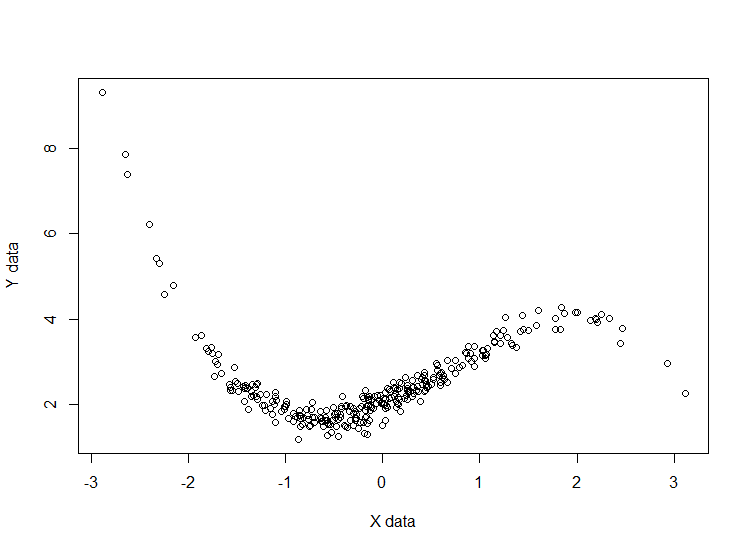
\includegraphics[width=\textwidth]{resources/q1_2_img1.png}
					\caption{Plot with points}
				\end{center}
			\end{figure}
			\item
			Create a new $X$ matrix that includes a column of 1s for an intercept, a column for the original $X$ values, and a column of polynomials for each $X^{i}$ for $i \in {2,3,4,5}$. This will create a matrix with dimensions $300 \times 6$.
			\begin{verbatim}
> x_data <- cbind(rep(1,300),data["X"],data["X"]^2,data["X"]^3,data["X"]^4,data["X"]^5)
> names(x_data) <- c("X0","X1","X2","X3","X4","X5")
			\end{verbatim}

			\item
			Find the OLS solution to this using $(X^{T}X)^{-1} X^{T}Y$.

\begin{lstlisting}[language=R,frame=single]
> xt <- t(x_data)
> xtx <- as.matrix(xt) %*% t(xt)
> xty <- as.matrix(xt) %*% as.matrix(data["Y"])
> beta <- solve(xtx) %*% xty
> beta
               Y
X0  2.0142724145
X1  0.9522479087
X2  0.5014464975
X3 -0.2219555459
X4  0.0001422326
X5 -0.0031247916
\end{lstlisting}
		\textbf{Note:} Here $X0$ is the intercept while $X1,X2,X3,X4,X5$ denote powers of $X$ etc.

		\item
		Overlay the fitted values (i.e. $X\hat{\beta}_{OLS}$) as a line on the plot of $Y$ vs. $X$.
		\begin{lstlisting}[language=R,frame=single]
> xpred <-  mapply("*",t(beta),x_data)
> y_pred <- rowSums(xpred)
> pred<- cbind(y_pred,x_data[2])
> pred_out <- arrange(pred,X1)
> plot(data[["X"]],data[["Y"]],xlab="X data",ylab="Y data")
> lines(pred_out$X1,pred_out$y_pred,col="red")
		\end{lstlisting}
		\begin{figure}[H]
				\begin{center}
					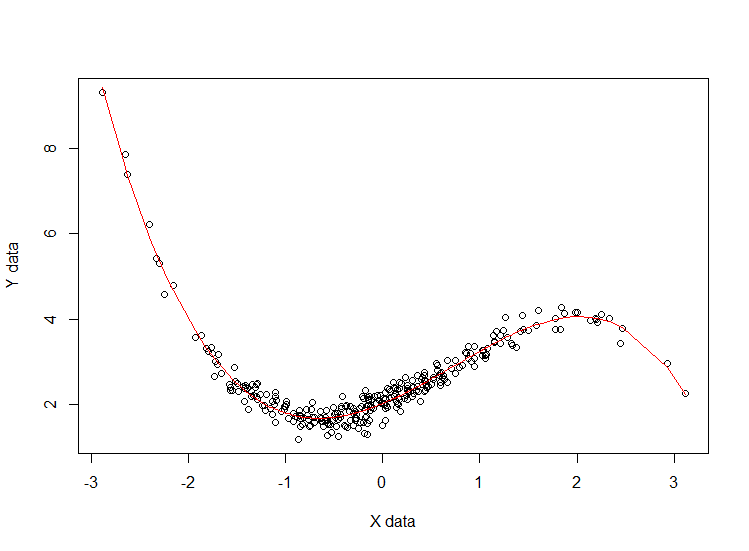
\includegraphics[width=\textwidth]{resources/q1_2_img2.png}
					\caption{Plot with points and overlaid line}
				\end{center}
			\end{figure}
		\end{itemize}
	\end{enumerate}

	\section{Question 2 [30 Points] - Artificial Neural Network}

	Consider the dataset Image Segmentation Data Set from the UCI repository \url{http://archive.ics.uci.edu/ml/datasets/Image+Segmentation}. The dataset consists of 19 precomputed attributes of 7 outdoor images, or 7 classes. You are provided with a training set and a test set. 

	Unlike the problems you are seen in the past, which have all been binary classification, this problem has seven classes. With Artificial Neural Network, there are at least 2 ways to construct a multi-class classifier:

	\begin{enumerate}
		\item
		Direct approach, where there are 7 output nodes to a neural network

		\item
		One-vs-All classification, where you build one binary classifier per class for each of the 7 classes. When predicting the correct class for a given instance in the test data, we choose the classifier that has the highest confidence.

		I did this using MultiClassClassifier and Multilayer Perceptron. By looking up on the internet I was able to find that setting certain values for momentum and learning rate was the best way to go. I wrote a piece of Javacode that loops thrugh various values for hidden layers, training time, learning rate and momentum. It picks up the best value for each and tries to pick the best value for the next attribute. The code and its output are listed below.
		The accuracy on the test set using this approach is $92.4286\%$

		\textbf{Accuracy : 92.4286\%}


	\end{enumerate}

	Your task is to build the best possible 7-output ANN and the best possible One-vs-All classifier. You must submit the following:

	\begin{itemize}
		\item
		A description of how you built the classifiers including the parameters you chose and the reason behind such a choice. The parameters include epoch, momentum, learning rate, number of hidden nodes and any other parameter you think might help.

		I used the multiLayer Perceptronin Weka for the Direct Approach. When trying to find values for the number of hidden nodes, I did a bit fo searching to see what would be th optimum number of nodes to choose and came across this article at \url{ftp://ftp.sas.com/pub/neural/FAQ3.html#A_hu}. After reading it I tried their suggestion of choosing the number of nodes as $( inputs + outputs) * \frac{2}{3}$. Thus the number of hidden nodes was chosen to be 17.
		Similarly I found values suggested for momentum, training time etc. I set up an array with all these values.

		I wrote Java code to use WEKA to loop through and find the best values for hidden layers, training time, learning rate and momentum when using the training set and using Cross Validation. I tried both a chained input and non chained. (Here chained refers to using the best value of hiddenlayers to find the best value for tarining time and so on). Once I was able to come up with the lowest possible error using CV on the training set, I used the WEKA GUI to run the parameters on the test set to see the accuracy on the test set.

		The reason for choice of the parameters was primarily to improve accuracy on CV and therefor hope to improve accuracy on test set. Some parameters like momentum etc have values which various websites mention as values that could be tried for various reasons.

		For one vs all the same technique was used excpect that a multilayerPerceptron was used with a MultiClassClassifier. Here however I ran the loops using the Weka Java API. After which I decided to try what would happen with 2 hidden layers. So keeping th best values of all values I changed Hidden layers to ``10,2''. This however seemd to make th accuracy go down. I after tinkering a bit i noticed that the momentum had to be changed as the model was probably settling on a local saddle point

		Note that program sometimes has many same accuracies on CV for any of the attributes. In this case all of them are tested to see which one is best.

		\textbf{Direct Parameters} \\
		Chose Learning Rate as ->0.1 \\
		Chose Hidden Layers as ->30 \\
		Chose Momentum as ->0.15 \\
		Chose training as ->1000 \\
		Accuracy on Test Set : 92.19\% \\

		\textbf{One Vs All Parameters}
		Chose Learning Rate as ->0.35 \\
		Chose Hidden Layers as ->``10,2'' \\
		Chose Momentum as ->0.2 \\
		Chose training as ->1000 \\
		Accuracy on Test Set : 92.19\% \\

		The output in 2 diffrent cases is given below. Program in code section below.

\begin{verbatim}
CV Direct Non chained

run:
FOR Learning ->0.05 
---------------------------
Correctly Classified Instances         183               87.1429 %
Incorrectly Classified Instances        27               12.8571 %
Kappa statistic                          0.85  
Mean absolute error                      0.057 
Root mean squared error                  0.1517
Relative absolute error                 23.2803 %
Root relative squared error             43.3575 %
Total Number of Instances              210     

FOR Learning ->0.1 
---------------------------
Correctly Classified Instances         189               90      %
Incorrectly Classified Instances        21               10      %
Kappa statistic                          0.8833
Mean absolute error                      0.0489
Root mean squared error                  0.1479
Relative absolute error                 19.9645 %
Root relative squared error             42.2619 %
Total Number of Instances              210     

FOR Learning ->0.15 
---------------------------
Correctly Classified Instances         189               90      %
Incorrectly Classified Instances        21               10      %
Kappa statistic                          0.8833
Mean absolute error                      0.0424
Root mean squared error                  0.1499
Relative absolute error                 17.2991 %
Root relative squared error             42.8333 %
Total Number of Instances              210     

FOR Learning ->0.2 
---------------------------
Correctly Classified Instances         187               89.0476 %
Incorrectly Classified Instances        23               10.9524 %
Kappa statistic                          0.8722
Mean absolute error                      0.043 
Root mean squared error                  0.1454
Relative absolute error                 17.5665 %
Root relative squared error             41.5579 %
Total Number of Instances              210     

FOR Learning ->0.25 
---------------------------
Correctly Classified Instances         185               88.0952 %
Incorrectly Classified Instances        25               11.9048 %
Kappa statistic                          0.8611
Mean absolute error                      0.0419
Root mean squared error                  0.1587
Relative absolute error                 17.101  %
Root relative squared error             45.3524 %
Total Number of Instances              210     

FOR Learning ->0.3 
---------------------------
Correctly Classified Instances         183               87.1429 %
Incorrectly Classified Instances        27               12.8571 %
Kappa statistic                          0.85  
Mean absolute error                      0.044 
Root mean squared error                  0.1613
Relative absolute error                 17.9846 %
Root relative squared error             46.104  %
Total Number of Instances              210     

FOR Learning ->0.35 
---------------------------
Correctly Classified Instances         187               89.0476 %
Incorrectly Classified Instances        23               10.9524 %
Kappa statistic                          0.8722
Mean absolute error                      0.0432
Root mean squared error                  0.162 
Relative absolute error                 17.6571 %
Root relative squared error             46.2961 %
Total Number of Instances              210     

FOR Learning ->0.4 
---------------------------
Correctly Classified Instances         183               87.1429 %
Incorrectly Classified Instances        27               12.8571 %
Kappa statistic                          0.85  
Mean absolute error                      0.0442
Root mean squared error                  0.1681
Relative absolute error                 18.0383 %
Root relative squared error             48.0418 %
Total Number of Instances              210     

FOR Learning ->0.9 
---------------------------
Correctly Classified Instances         185               88.0952 %
Incorrectly Classified Instances        25               11.9048 %
Kappa statistic                          0.8611
Mean absolute error                      0.0423
Root mean squared error                  0.1717
Relative absolute error                 17.2658 %
Root relative squared error             49.0555 %
Total Number of Instances              210     

Choosing Learning Rate as ->0.1
For Hidden ->5 
---------------------------
Correctly Classified Instances         183               87.1429 %
Incorrectly Classified Instances        27               12.8571 %
Kappa statistic                          0.85  
Mean absolute error                      0.0523
Root mean squared error                  0.1765
Relative absolute error                 21.3532 %
Root relative squared error             50.4403 %
Total Number of Instances              210     

For Hidden ->10 
---------------------------
Correctly Classified Instances         184               87.619  %
Incorrectly Classified Instances        26               12.381  %
Kappa statistic                          0.8556
Mean absolute error                      0.0463
Root mean squared error                  0.1626
Relative absolute error                 18.924  %
Root relative squared error             46.464  %
Total Number of Instances              210     

For Hidden ->12 
---------------------------
Correctly Classified Instances         184               87.619  %
Incorrectly Classified Instances        26               12.381  %
Kappa statistic                          0.8556
Mean absolute error                      0.0436
Root mean squared error                  0.1604
Relative absolute error                 17.7989 %
Root relative squared error             45.8419 %
Total Number of Instances              210     

For Hidden ->17 
---------------------------
Correctly Classified Instances         186               88.5714 %
Incorrectly Classified Instances        24               11.4286 %
Kappa statistic                          0.8667
Mean absolute error                      0.0423
Root mean squared error                  0.1597
Relative absolute error                 17.2884 %
Root relative squared error             45.6387 %
Total Number of Instances              210     

For Hidden ->20 
---------------------------
Correctly Classified Instances         187               89.0476 %
Incorrectly Classified Instances        23               10.9524 %
Kappa statistic                          0.8722
Mean absolute error                      0.0425
Root mean squared error                  0.1617
Relative absolute error                 17.346  %
Root relative squared error             46.2216 %
Total Number of Instances              210     

For Hidden ->30 
---------------------------
Correctly Classified Instances         191               90.9524 %
Incorrectly Classified Instances        19                9.0476 %
Kappa statistic                          0.8944
Mean absolute error                      0.0378
Root mean squared error                  0.151 
Relative absolute error                 15.4241 %
Root relative squared error             43.1599 %
Total Number of Instances              210     

For Hidden ->a 
---------------------------
Correctly Classified Instances         184               87.619  %
Incorrectly Classified Instances        26               12.381  %
Kappa statistic                          0.8556
Mean absolute error                      0.0452
Root mean squared error                  0.1674
Relative absolute error                 18.4435 %
Root relative squared error             47.8406 %
Total Number of Instances              210     

Choosing Hidden Layers as ->30
For Momentum ->0.05 
---------------------------
Correctly Classified Instances         184               87.619  %
Incorrectly Classified Instances        26               12.381  %
Kappa statistic                          0.8556
Mean absolute error                      0.0415
Root mean squared error                  0.1532
Relative absolute error                 16.9534 %
Root relative squared error             43.7935 %
Total Number of Instances              210     

For Momentum ->0.1 
---------------------------
Correctly Classified Instances         186               88.5714 %
Incorrectly Classified Instances        24               11.4286 %
Kappa statistic                          0.8667
Mean absolute error                      0.043 
Root mean squared error                  0.1628
Relative absolute error                 17.5506 %
Root relative squared error             46.5356 %
Total Number of Instances              210     

For Momentum ->0.15 
---------------------------
Correctly Classified Instances         190               90.4762 %
Incorrectly Classified Instances        20                9.5238 %
Kappa statistic                          0.8889
Mean absolute error                      0.0388
Root mean squared error                  0.1495
Relative absolute error                 15.8378 %
Root relative squared error             42.7351 %
Total Number of Instances              210     

For Momentum ->0.2 
---------------------------
Correctly Classified Instances         188               89.5238 %
Incorrectly Classified Instances        22               10.4762 %
Kappa statistic                          0.8778
Mean absolute error                      0.0388
Root mean squared error                  0.1566
Relative absolute error                 15.8384 %
Root relative squared error             44.7443 %
Total Number of Instances              210     

For Momentum ->0.25 
---------------------------
Correctly Classified Instances         189               90      %
Incorrectly Classified Instances        21               10      %
Kappa statistic                          0.8833
Mean absolute error                      0.0392
Root mean squared error                  0.153 
Relative absolute error                 15.9983 %
Root relative squared error             43.7092 %
Total Number of Instances              210     

For Momentum ->0.3 
---------------------------
Correctly Classified Instances         184               87.619  %
Incorrectly Classified Instances        26               12.381  %
Kappa statistic                          0.8556
Mean absolute error                      0.0439
Root mean squared error                  0.1639
Relative absolute error                 17.9291 %
Root relative squared error             46.8501 %
Total Number of Instances              210     

For Momentum ->0.9 
---------------------------
Correctly Classified Instances         187               89.0476 %
Incorrectly Classified Instances        23               10.9524 %
Kappa statistic                          0.8722
Mean absolute error                      0.037 
Root mean squared error                  0.1631
Relative absolute error                 15.1114 %
Root relative squared error             46.6227 %
Total Number of Instances              210     

Choosing Momentum as ->0.15
For Training ->50 
---------------------------
Correctly Classified Instances         187               89.0476 %
Incorrectly Classified Instances        23               10.9524 %
Kappa statistic                          0.8722
Mean absolute error                      0.0705
Root mean squared error                  0.1601
Relative absolute error                 28.7859 %
Root relative squared error             45.7629 %
Total Number of Instances              210     

For Training ->100 
---------------------------
Correctly Classified Instances         184               87.619  %
Incorrectly Classified Instances        26               12.381  %
Kappa statistic                          0.8556
Mean absolute error                      0.0544
Root mean squared error                  0.1601
Relative absolute error                 22.2004 %
Root relative squared error             45.7576 %
Total Number of Instances              210     

For Training ->250 
---------------------------
Correctly Classified Instances         185               88.0952 %
Incorrectly Classified Instances        25               11.9048 %
Kappa statistic                          0.8611
Mean absolute error                      0.0478
Root mean squared error                  0.1637
Relative absolute error                 19.5089 %
Root relative squared error             46.7937 %
Total Number of Instances              210     

For Training ->500 
---------------------------
Correctly Classified Instances         186               88.5714 %
Incorrectly Classified Instances        24               11.4286 %
Kappa statistic                          0.8667
Mean absolute error                      0.0408
Root mean squared error                  0.1609
Relative absolute error                 16.6718 %
Root relative squared error             45.9951 %
Total Number of Instances              210     

For Training ->750 
---------------------------
Correctly Classified Instances         188               89.5238 %
Incorrectly Classified Instances        22               10.4762 %
Kappa statistic                          0.8778
Mean absolute error                      0.04  
Root mean squared error                  0.1623
Relative absolute error                 16.328  %
Root relative squared error             46.3705 %
Total Number of Instances              210     

For Training ->1000 
---------------------------
Correctly Classified Instances         191               90.9524 %
Incorrectly Classified Instances        19                9.0476 %
Kappa statistic                          0.8944
Mean absolute error                      0.0367
Root mean squared error                  0.1517
Relative absolute error                 14.9992 %
Root relative squared error             43.3591 %
Total Number of Instances              210     

For Training ->5000 
---------------------------
Correctly Classified Instances         186               88.5714 %
Incorrectly Classified Instances        24               11.4286 %
Kappa statistic                          0.8667
Mean absolute error                      0.0384
Root mean squared error                  0.1707
Relative absolute error                 15.6778 %
Root relative squared error             48.7884 %
Total Number of Instances              210     

Final Choices of Values 

-------------------------------------
Chose Learning Rate as ->0.1
Chose Hidden Layers as ->30
Chose Momentum as ->0.15
Chose training as ->1000
BUILD SUCCESSFUL (total time: 4 minutes 50 seconds)

\end{verbatim}
\begin{verbatim}
CV One Vs ALL Non Chained
run:
FOR Learning ->0.05 
---------------------------
Correctly Classified Instances         190               90.4762 %
Incorrectly Classified Instances        20                9.5238 %
Kappa statistic                          0.8889
Mean absolute error                      0.2342
Root mean squared error                  0.3347
Relative absolute error                 95.6208 %
Root relative squared error             95.6426 %
Total Number of Instances              210     

FOR Learning ->0.1 
---------------------------
Correctly Classified Instances         185               88.0952 %
Incorrectly Classified Instances        25               11.9048 %
Kappa statistic                          0.8611
Mean absolute error                      0.234 
Root mean squared error                  0.3344
Relative absolute error                 95.5317 %
Root relative squared error             95.5569 %
Total Number of Instances              210     

FOR Learning ->0.15 
---------------------------
Correctly Classified Instances         187               89.0476 %
Incorrectly Classified Instances        23               10.9524 %
Kappa statistic                          0.8722
Mean absolute error                      0.2339
Root mean squared error                  0.3344
Relative absolute error                 95.5219 %
Root relative squared error             95.5503 %
Total Number of Instances              210     

FOR Learning ->0.2 
---------------------------
Correctly Classified Instances         190               90.4762 %
Incorrectly Classified Instances        20                9.5238 %
Kappa statistic                          0.8889
Mean absolute error                      0.2338
Root mean squared error                  0.3341
Relative absolute error                 95.4544 %
Root relative squared error             95.4813 %
Total Number of Instances              210     

FOR Learning ->0.25 
---------------------------
Correctly Classified Instances         188               89.5238 %
Incorrectly Classified Instances        22               10.4762 %
Kappa statistic                          0.8778
Mean absolute error                      0.2336
Root mean squared error                  0.3339
Relative absolute error                 95.3806 %
Root relative squared error             95.4062 %
Total Number of Instances              210     

FOR Learning ->0.3 
---------------------------
Correctly Classified Instances         192               91.4286 %
Incorrectly Classified Instances        18                8.5714 %
Kappa statistic                          0.9   
Mean absolute error                      0.2337
Root mean squared error                  0.334 
Relative absolute error                 95.4189 %
Root relative squared error             95.4453 %
Total Number of Instances              210     

FOR Learning ->0.35 
---------------------------
Correctly Classified Instances         193               91.9048 %
Incorrectly Classified Instances        17                8.0952 %
Kappa statistic                          0.9056
Mean absolute error                      0.2335
Root mean squared error                  0.3337
Relative absolute error                 95.3354 %
Root relative squared error             95.3626 %
Total Number of Instances              210     

FOR Learning ->0.4 
---------------------------
Correctly Classified Instances         189               90      %
Incorrectly Classified Instances        21               10      %
Kappa statistic                          0.8833
Mean absolute error                      0.2335
Root mean squared error                  0.3337
Relative absolute error                 95.3273 %
Root relative squared error             95.3548 %
Total Number of Instances              210     

FOR Learning ->0.9 
---------------------------
Correctly Classified Instances         185               88.0952 %
Incorrectly Classified Instances        25               11.9048 %
Kappa statistic                          0.8611
Mean absolute error                      0.2336
Root mean squared error                  0.3339
Relative absolute error                 95.3949 %
Root relative squared error             95.4251 %
Total Number of Instances              210     

Choosing Learning Rate as ->0.35
For Hidden ->5 
---------------------------
Correctly Classified Instances         189               90      %
Incorrectly Classified Instances        21               10      %
Kappa statistic                          0.8833
Mean absolute error                      0.2335
Root mean squared error                  0.3338
Relative absolute error                 95.3608 %
Root relative squared error             95.3902 %
Total Number of Instances              210     

For Hidden ->10 
---------------------------
Correctly Classified Instances         188               89.5238 %
Incorrectly Classified Instances        22               10.4762 %
Kappa statistic                          0.8778
Mean absolute error                      0.2336
Root mean squared error                  0.3339
Relative absolute error                 95.3942 %
Root relative squared error             95.4206 %
Total Number of Instances              210     

For Hidden ->12 
---------------------------
Correctly Classified Instances         188               89.5238 %
Incorrectly Classified Instances        22               10.4762 %
Kappa statistic                          0.8778
Mean absolute error                      0.2336
Root mean squared error                  0.3339
Relative absolute error                 95.3867 %
Root relative squared error             95.417  %
Total Number of Instances              210     

For Hidden ->17 
---------------------------
Correctly Classified Instances         189               90      %
Incorrectly Classified Instances        21               10      %
Kappa statistic                          0.8833
Mean absolute error                      0.2335
Root mean squared error                  0.3337
Relative absolute error                 95.353  %
Root relative squared error             95.3754 %
Total Number of Instances              210     

For Hidden ->20 
---------------------------
Correctly Classified Instances         187               89.0476 %
Incorrectly Classified Instances        23               10.9524 %
Kappa statistic                          0.8722
Mean absolute error                      0.2337
Root mean squared error                  0.334 
Relative absolute error                 95.4289 %
Root relative squared error             95.4534 %
Total Number of Instances              210     

For Hidden ->30 
---------------------------
Correctly Classified Instances         189               90      %
Incorrectly Classified Instances        21               10      %
Kappa statistic                          0.8833
Mean absolute error                      0.2337
Root mean squared error                  0.3341
Relative absolute error                 95.44   %
Root relative squared error             95.4679 %
Total Number of Instances              210     

For Hidden ->a 
---------------------------
Correctly Classified Instances         190               90.4762 %
Incorrectly Classified Instances        20                9.5238 %
Kappa statistic                          0.8889
Mean absolute error                      0.2336
Root mean squared error                  0.3339
Relative absolute error                 95.3858 %
Root relative squared error             95.4185 %
Total Number of Instances              210     

Choosing Hidden Layers as ->a
For Momentum ->0.05 
---------------------------
Correctly Classified Instances         187               89.0476 %
Incorrectly Classified Instances        23               10.9524 %
Kappa statistic                          0.8722
Mean absolute error                      0.2337
Root mean squared error                  0.334 
Relative absolute error                 95.4318 %
Root relative squared error             95.4588 %
Total Number of Instances              210     

For Momentum ->0.1 
---------------------------
Correctly Classified Instances         190               90.4762 %
Incorrectly Classified Instances        20                9.5238 %
Kappa statistic                          0.8889
Mean absolute error                      0.2336
Root mean squared error                  0.3338
Relative absolute error                 95.3795 %
Root relative squared error             95.4052 %
Total Number of Instances              210     

For Momentum ->0.15 
---------------------------
Correctly Classified Instances         188               89.5238 %
Incorrectly Classified Instances        22               10.4762 %
Kappa statistic                          0.8778
Mean absolute error                      0.2338
Root mean squared error                  0.3341
Relative absolute error                 95.4552 %
Root relative squared error             95.4824 %
Total Number of Instances              210     

For Momentum ->0.2 
---------------------------
Correctly Classified Instances         186               88.5714 %
Incorrectly Classified Instances        24               11.4286 %
Kappa statistic                          0.8667
Mean absolute error                      0.2338
Root mean squared error                  0.3342
Relative absolute error                 95.4723 %
Root relative squared error             95.501  %
Total Number of Instances              210     

For Momentum ->0.25 
---------------------------
Correctly Classified Instances         188               89.5238 %
Incorrectly Classified Instances        22               10.4762 %
Kappa statistic                          0.8778
Mean absolute error                      0.2338
Root mean squared error                  0.3342
Relative absolute error                 95.466  %
Root relative squared error             95.4967 %
Total Number of Instances              210     

For Momentum ->0.3 
---------------------------
Correctly Classified Instances         191               90.9524 %
Incorrectly Classified Instances        19                9.0476 %
Kappa statistic                          0.8944
Mean absolute error                      0.2337
Root mean squared error                  0.3341
Relative absolute error                 95.4363 %
Root relative squared error             95.463  %
Total Number of Instances              210     

For Momentum ->0.9 
---------------------------
Correctly Classified Instances         183               87.1429 %
Incorrectly Classified Instances        27               12.8571 %
Kappa statistic                          0.85  
Mean absolute error                      0.2341
Root mean squared error                  0.3346
Relative absolute error                 95.5844 %
Root relative squared error             95.6219 %
Total Number of Instances              210     

Choosing Momentum as ->0.3
For Training ->50 
---------------------------
Correctly Classified Instances         189               90      %
Incorrectly Classified Instances        21               10      %
Kappa statistic                          0.8833
Mean absolute error                      0.2347
Root mean squared error                  0.3354
Relative absolute error                 95.8259 %
Root relative squared error             95.8485 %
Total Number of Instances              210     

For Training ->100 
---------------------------
Correctly Classified Instances         187               89.0476 %
Incorrectly Classified Instances        23               10.9524 %
Kappa statistic                          0.8722
Mean absolute error                      0.2342
Root mean squared error                  0.3348
Relative absolute error                 95.6388 %
Root relative squared error             95.663  %
Total Number of Instances              210     

For Training ->250 
---------------------------
Correctly Classified Instances         190               90.4762 %
Incorrectly Classified Instances        20                9.5238 %
Kappa statistic                          0.8889
Mean absolute error                      0.2338
Root mean squared error                  0.3341
Relative absolute error                 95.453  %
Root relative squared error             95.4775 %
Total Number of Instances              210     

For Training ->500 
---------------------------
Correctly Classified Instances         190               90.4762 %
Incorrectly Classified Instances        20                9.5238 %
Kappa statistic                          0.8889
Mean absolute error                      0.2337
Root mean squared error                  0.334 
Relative absolute error                 95.4337 %
Root relative squared error             95.4609 %
Total Number of Instances              210     

For Training ->750 
---------------------------
Correctly Classified Instances         191               90.9524 %
Incorrectly Classified Instances        19                9.0476 %
Kappa statistic                          0.8944
Mean absolute error                      0.2336
Root mean squared error                  0.3339
Relative absolute error                 95.3783 %
Root relative squared error             95.4063 %
Total Number of Instances              210     

For Training ->1000 
---------------------------
Correctly Classified Instances         193               91.9048 %
Incorrectly Classified Instances        17                8.0952 %
Kappa statistic                          0.9056
Mean absolute error                      0.2335
Root mean squared error                  0.3337
Relative absolute error                 95.3391 %
Root relative squared error             95.365  %
Total Number of Instances              210     

For Training ->5000 
---------------------------
Correctly Classified Instances         187               89.0476 %
Incorrectly Classified Instances        23               10.9524 %
Kappa statistic                          0.8722
Mean absolute error                      0.2337
Root mean squared error                  0.3341
Relative absolute error                 95.4463 %
Root relative squared error             95.4827 %
Total Number of Instances              210     

Final Choices of Values 

-------------------------------------
Chose Learning Rate as ->0.35
Chose Hidden Layers as ->a
Chose training as ->1000
Chose Momentum as ->0.3
BUILD SUCCESSFUL (total time: 19 minutes 40 seconds)

\end{verbatim}
		\item
		A descriptive comparison in performance between the 7-output ANN and the One-vs-All ANN - compare the 2 models based on their predictive performance on the given test data, training time, and your judgment of which approach is better for this problem.

		Considerign the fact that I was able to achieve the same accruacy on the training set with both models, commenting on the predictive performance is harder. However it can be noted that with a varied se of attributes the overall accuracy by the One Vs All seems to be better.

		In terms of training time it easily noted by the run time taken in Java that the th time taken by the One Vs All method is almost 5 times that of the direct approach.

		I think that if it is ok to slightly compromise a very small amount on accuracy the direct approach should be used because it is MUCH faster than the other.
		\item
		Any code you have written (using Matlab, R, Weka’s Java API)
\begin{lstlisting}[language=Java,frame=single]
/*
 * To change this template, choose Tools | Templates
 * and open the template in the editor.
 */
package wekacode;
import java.util.Random;
import weka.classifiers.Classifier;
import weka.classifiers.Evaluation;
import weka.classifiers.functions.MultilayerPerceptron;
import weka.core.Instances;
import weka.core.converters.ConverterUtils.DataSource;
import weka.classifiers.meta.MultiClassClassifier;
import weka.core.Attribute;
import weka.core.SelectedTag;
import weka.core.Tag;
/**
 *
 * @author Roopak
 */
public class WekaCode {

    /**
     * @param args the command line arguments
     */
    int direct=0;
    int vary_learning=0;
    double vlearning[] = {0.05,0.1,0.15,0.2,0.25,0.3,0.35,0.4,0.9};
    
    int vary_hidden_layers=0;
    String vhidden[] = {"5","10","12","17","20","30","a"};
    
    int vary_momentum=0;
    double vmomentum[] = {0.05,0.1,0.15,0.2,0.25,0.3,0.9};
    
    int vary_training_time=0;
    int vtraining[] = {50,100,250,500,750,1000,5000};
    
    Instances train,test;
    DataSource source,source2;
    public WekaCode() throws Exception
    {
        source = new DataSource("D:\\Courses\\data_mining - "
                +"CSC522\\homework\\hw5\\segmentation.arff");
        train = source.getDataSet();
        //Attribute a = new Attribute("CLASS");
        train.setClassIndex(0);
        
        source2 = new DataSource("D:\\Courses\\data_mining - "
                +"CSC522\\homework\\hw5\\segmentation.test.arff");
        test = source2.getDataSet();
        test.setClassIndex(0);
    }
    public void q2_p1() throws Exception
    {
        
    }
    
    public void q2_p2() throws Exception
    {
        
        MultilayerPerceptron mlp = new MultilayerPerceptron();
        mlp.setValidationSetSize(0);
        mlp.setValidationThreshold(20);
        mlp.setNominalToBinaryFilter(true);
        mlp.setNormalizeAttributes(true);
        mlp.setNormalizeNumericClass(true);
        mlp.setReset(true);
        
        mlp.setDebug(false);
        mlp.setGUI(false);
        mlp.setDecay(false);
        mlp.setAutoBuild(true);
        
        double temp;
        double maxlrn=0;
        double bestlrn=0.3;
        if(vary_learning==1)
        {
            for(int counter=0; counter < vlearning.length;counter++)
            {
                mlp.setMomentum(0.2);
                mlp.setTrainingTime(500);
                mlp.setHiddenLayers("a");
                
                mlp.setLearningRate(vlearning[counter]);
                temp=train_and_predict(mlp, "FOR Learning ->" 
                        + vlearning[counter] + " \n---------------------------");
                if(temp>maxlrn)
                {
                    maxlrn = temp;
                    bestlrn = vlearning[counter];
                }
            }
        }
        
        System.out.println("Choosing Learning Rate as ->" + bestlrn);
        double maxhidden=0;
        String besthidden="a";
        if(vary_hidden_layers==1)
        {
            for(int counter=0; counter < vhidden.length;counter++)
            {
                mlp.setMomentum(0.2);
                mlp.setTrainingTime(500);
                mlp.setLearningRate(0.3);
                
                mlp.setHiddenLayers(vhidden[counter]);
                temp = train_and_predict(mlp, "For Hidden ->" 
                        + vhidden[counter] + " \n---------------------------");
                if(temp>maxhidden)
                {
                    maxhidden = temp;
                    besthidden = vhidden[counter];
                }
            }
        }
        
        System.out.println("Choosing Hidden Layers as ->" + besthidden);
        double maxmom=0;
        double bestmom=0.2;
        if(vary_momentum==1)
        {
            for(int counter=0; counter < vmomentum.length;counter++)
            {
                mlp.setTrainingTime(500);
                mlp.setLearningRate(0.3);
                mlp.setHiddenLayers("a");
                
                mlp.setMomentum(vmomentum[counter]);
                temp = train_and_predict(mlp, "For Momentum ->" 
                        + vmomentum[counter] + " \n---------------------------");
                if(temp>maxmom)
                {
                    maxmom=temp;
                    bestmom=vmomentum[counter];
                }
            }
        }
        
        System.out.println("Choosing Momentum as ->" + bestmom);
        double maxtt=0;
        int besttt=500;
        if(vary_training_time==1)
        {
            for(int counter=0; counter < vtraining.length;counter++)
            {
                mlp.setLearningRate(0.3);
                mlp.setHiddenLayers("a");
                mlp.setMomentum(0.2);
                
                mlp.setTrainingTime(vtraining[counter]);
                temp = train_and_predict(mlp, "For Training ->" 
                        + vtraining[counter] + " \n---------------------------");
                if(temp>maxtt)
                {
                    maxtt=temp;
                    besttt=vtraining[counter];
                }
            }
        }
        
        System.out.println("Final Choices of Values \n");
        System.out.println("-------------------------------------");
        System.out.println("Chose Learning Rate as ->" + bestlrn);
        System.out.println("Chose Hidden Layers as ->" + besthidden);
        System.out.println("Chose Momentum as ->" + bestmom);
        System.out.println("Chose training as ->" + besttt);
        
    }
    public double train_and_predict(MultilayerPerceptron mlp,String title)
            throws Exception
    {
        if(direct==1)
        {
            return train_and_predict_single(mlp,title);
        }
        MultiClassClassifier c1;
        c1 = new MultiClassClassifier();
        c1.setClassifier(mlp);
        
        
        Random rand = new Random();
        Instances randData = new Instances(train);
        randData.randomize(rand);
        if (randData.classAttribute().isNominal())
            randData.stratify(10);
        
        Evaluation eval = new Evaluation(randData);
         for (int n = 0; n < 10; n++)
         {
            Instances mytrain = randData.trainCV(10, n);
            Instances mytest = randData.testCV(10, n);

            MultiClassClassifier clsCopy = new MultiClassClassifier();
            clsCopy.setClassifier(mlp);
            clsCopy.buildClassifier(mytrain);
            eval.evaluateModel(clsCopy, mytest);
         }
        
        //c1.buildClassifier(train);
        //Evaluation eval = new Evaluation(train);
        //eval.evaluateModel(c1, test) ;
        
        //eval.
        //eval.
        System.out.println(eval.toSummaryString(title, false));
        return eval.pctCorrect();
        
    }
    public double train_and_predict_single(MultilayerPerceptron mlp,String title)
            throws Exception
    {
        Classifier c1;
        c1 = mlp;
        
        Random rand = new Random();
        Instances randData = new Instances(train);
        randData.randomize(rand);
        if (randData.classAttribute().isNominal())
            randData.stratify(10);
        
        Evaluation eval = new Evaluation(randData);
         for (int n = 0; n < 10; n++)
         {
            Instances mytrain = randData.trainCV(10, n);
            Instances mytest = randData.testCV(10, n);

            Classifier clsCopy = Classifier.makeCopy(c1);
            clsCopy.buildClassifier(mytrain);
            eval.evaluateModel(clsCopy, mytest);
         }
        
        //c1.setClassifier(mlp);
        //Tag t[]= new Tag[1];
        //SelectedTag tg = new SelectedTag("1-against-all",new Tag[1]);
        //c1.setMethod(tg);
        
        //c1.buildClassifier(train);
        //Evaluation eval = new Evaluation(train);
        //eval.evaluateModel(c1, test) ;
        
        //eval.
        //eval.
        System.out.println(eval.toSummaryString(title, false));
        return eval.pctCorrect();
    }
    public static void main(String[] args) {
        // TODO code application logic here
       
        try
        {
            WekaCode a = new WekaCode();
            a.vary_hidden_layers=1;
            a.vary_learning=1;
            a.vary_momentum=1;
            a.vary_training_time=1;
            a.direct=1;
            a.q2_p2();
        }
        catch(Exception e)
        {
            e.printStackTrace();
        }
    }
}

\end{lstlisting}
	\end{itemize}

	\section{Question 3 [10 Points (6 + 4)] - Multi-Class Classification}


	An electronic nose is a device that can ``sniff'' gases at various locations. One way to construct the devise is using an array of $N$ semiconductors, each of which will have a different voltage response when in contact with certain gases. Each semiconductor responds to at least one gas (i.e., more than one gas). Let us assume that there are 3 gases A, B and C. Some locations can have either one of the gases or a mixture of gases. Thus, possible class labels are: A, B, C, AB, AC, BC, ABC.

	\begin{enumerate}
		\item
		If you are allowed to use only an Artificial Neural Network, which of the following con-figurations are possible? State why or why not.
		\begin{itemize}
			\item
			1 network with 7 output nodes.

			This would be the simple choice. The output nodes would be $A, B, C, AB, AC, BC, ABC$. Thus this configuration is possible. 
			\item
			One-vs-All

			This is again possible if we are trying to find presence of one vs others etc. So it could be $A$ present vs $A$ not present or maybe $AC$ present vs $AC$ not present

			\item
			1 network with only 3 output nodes

			Let us say we construct the neural network in such a way that we output the presence of any gas which the neural network says is present with a confidence of 70\% or more. Then we can use this neural network to give the output of gases in the various possibilities. Thus if say the network gives us that $A$ is present with a confidence of 89\% and say $C$ is present with 71\%. Then we can say that the gases present in the region are AC. Thus with three output nodes we can detect the presence of any of the possible combinations. Thus we can say that this network would be possible with 3 output nodes.
		\end{itemize}

		\item
		Irrespective of your answer for the previous part, for each of the above configurations, comment on the complexity of the network. Comment on how you would choose the number of hidden nodes, training time and number of epochs for each of the networks.

		The complexit of the network will vary. With a simple guess it is easy to say that the 1 network with 7 outputs could probably be the simplest while One vs All might be more comples as this would involve the construction of 7 networks and combining them to get the required output.

		Epoch represents when training will stop. Usually we can say that if highe enough this shouldnt be a problem. But in most cases having too high a value will just increase training time and not really have a positive benefit.

		hidden nodes - The article at \url{ftp://ftp.sas.com/pub/neural/FAQ3.html#A_hu} says we should try and have $( inputs + outputs) * \frac{2}{3}$ as the number of hidden nodes. Not however that many sources cite that it is best to not have more than 2 levels.

	\end{enumerate}

	\section{Question 4 [8 Points] - Hyperplanes for Classification}

	Consider $N$ points in a D-dimensional space, some of which are positive and some of which are negative. We all know that for $N = 2$ points in $d = 1$ dimensions, a line can separate positive and negative examples. Based on this, state whether a similar linear separator is possible for each of the following cases. If a linear separator is not possible, give an example and state conditions that must be satisfied for the existence of a linear classifier. The correct answer to this question considers all possible arrangements of the N points in the D-dimensional space. If a linear separator is not possible for even one such arrangement, your answer should state that case as an example for failure and state the conditions when a linear separator is possible. \\

	Note that a trivial case if I chose all points to lie at the same location or to lie on a line it is not possible to separate them.
	\begin{itemize}
		\item
		N=3, D=2

		\item
		N=4, D=2

		\item
		N=4, D=3

		\item
		N=5, D=3
	\end{itemize}
\end{document}